%%%%%%%% ICML 2026 SUBMISSION -- Distribution-Free Sequential Learning %%%%%%%%
% NOTE: icml2026.sty / icml2026.bst in this folder are LOCAL PREVIEW SHIMS.
% Replace them with the official ICML 2026 author-kit files before submitting.

\documentclass{article}

\usepackage{microtype}
\usepackage{graphicx}
\usepackage{subcaption}
\usepackage{booktabs}
\usepackage{hyperref}

\newcommand{\theHalgorithm}{\arabic{algorithm}}

% Blind version for review:
\usepackage{icml2026}

\usepackage{amsmath}
\usepackage{amssymb}
\usepackage{mathtools}
\usepackage{amsthm}
\usepackage{algorithm}
\usepackage{algorithmic}

\usepackage[capitalize,noabbrev]{cleveref}

\graphicspath{{figures/}}

%%%%%%%%%%%%%%%%%%%%%%%%%%%%%%%%
% THEOREMS
%%%%%%%%%%%%%%%%%%%%%%%%%%%%%%%%
% Shared numbering via thmtools `sibling=` so cleveref names each environment
% correctly (Assumption/Lemma/Remark/Proposition) instead of all ``Theorem''.
\usepackage{thmtools}
\declaretheorem[name=Theorem,numberwithin=section]{theorem}
\declaretheorem[name=Proposition,sibling=theorem]{proposition}
\declaretheorem[name=Lemma,sibling=theorem]{lemma}
\declaretheorem[name=Corollary,sibling=theorem]{corollary}
\declaretheorem[name=Definition,sibling=theorem,style=definition]{definition}
\declaretheorem[name=Assumption,sibling=theorem,style=definition]{assumption}
\declaretheorem[name=Remark,sibling=theorem,style=remark]{remark}
\crefname{theorem}{Theorem}{Theorems}
\crefname{proposition}{Proposition}{Propositions}
\crefname{lemma}{Lemma}{Lemmas}
\crefname{corollary}{Corollary}{Corollaries}
\crefname{definition}{Definition}{Definitions}
\crefname{assumption}{Assumption}{Assumptions}
\crefname{remark}{Remark}{Remarks}

% Math shorthands
\newcommand{\E}{\mathbb{E}}
\newcommand{\R}{\mathbb{R}}
\newcommand{\N}{\mathbb{N}}
\newcommand{\ip}[2]{\langle #1, #2 \rangle}
\newcommand{\norm}[1]{\lVert #1 \rVert}
\newcommand{\gt}{g_t}
\newcommand{\clip}{\operatorname{clip}}
\DeclareMathOperator*{\argmin}{arg\,min}

\icmltitlerunning{Nonstationarity Manufactures Heavy Tails}

\begin{document}

\twocolumn[
  \icmltitle{Nonstationarity Manufactures Heavy Tails:\\ Scale-Normalized Sequential Learning}

  \icmlsetsymbol{equal}{*}
  \begin{icmlauthorlist}
    \icmlauthor{Anonymous Authors}{yyy}
  \end{icmlauthorlist}
  \icmlaffiliation{yyy}{Anonymous Institution}
  \icmlcorrespondingauthor{Anonymous}{anon@example.com}
  \icmlkeywords{online learning, nonstationarity, scale normalization, heavy tails, dynamic regret}
  \vskip 0.3in
]

\printAffiliationsAndNotice{}

\begin{abstract}
We study online prediction on streams whose loss-gradient \emph{scale} is strongly
nonstationary, using a large financial dataset as a testbed. The gradient-norm scale
drifts several-fold across the record with overnight jumps, and this drift alone makes
the \emph{pooled} gradient look heavy-tailed (tail index $\hat\alpha\approx2.4$); the
\emph{causally scale-normalized} gradient---the quantity a learner should actually act
on---is markedly lighter ($\hat\alpha\approx3.7$), so the difficulty is dominated by
nonstationarity rather than by an intrinsically heavy tail. In this regime plain online
gradient descent (OGD) has no usable learning rate---small rates underfit while any rate
large enough to learn diverges when the scale spikes---and clipping to a
\emph{scale-dependent} threshold is fragile because the clipped step still inherits the
drift. We propose \emph{Scale-Normalized OMD} (SN-OMD), which divides the gradient by a
tracked robust scale and caps it at a \emph{scale-free} constant $M$; the per-step move
is then bounded by $M$ rather than by a regime-dependent quantity, so the iterates
provably remain bounded for any learning rate or realization (a stability, not
convergence, guarantee). We prove a high-probability dynamic-regret bound of order
$T^{1/p}$ under a finite, possibly time-varying $p$-th moment ($p\in(1,2]$), and give a
budget calculation---corroborated by a direct measurement---indicating that the
interaction of tail drift with a moving comparator pushes \emph{dynamic} regret well
above $\sqrt T$. Empirically, on a continuous multi-regime stream SN-OMD stays bounded
across the entire tested learning-rate range and is the most accurate of the methods
compared, whereas OGD and scale-dependent clipping both diverge above
$\mathrm{lr}=10^{-2}$.
\end{abstract}

\section{Introduction}
\label{sec:intro}

Financial markets are a canonical source of heavy-tailed, distribution-free data:
returns and microstructure signals exhibit power-law tails, occasional data errors
act as adversarial contamination, and assumptions such as sub-Gaussianity are
untenable. Sequential prediction on such streams therefore calls for
\emph{distribution-free} guarantees that hold under weak moment assumptions only.
A rich line of work in robust statistics shows that the empirical mean is a poor
estimator under heavy tails, whereas estimators such as Catoni's M-estimator,
median-of-means, and the trimmed mean achieve sub-Gaussian deviations assuming only a
finite variance \citep{catoni2012,devroye2016,lugosi2019}; in optimization, gradient
clipping is the corresponding algorithmic primitive for heavy-tailed gradient noise
\citep{zhang2020clip,gorbunov2020,nguyen2023}.

This paper concerns a facet these lines mostly abstract away: on real streams the
gradient \emph{scale} is strongly nonstationary, and this---more than an intrinsically
heavy tail---is what breaks existing methods. Measuring the gradient of an online linear
predictor on the Jane Street market dataset, we find (i) the gradient \emph{scale}
drifts roughly $6\times$ across two months with overnight jumps; (ii) this drift alone
inflates the \emph{pooled} gradient-norm tail index to $\hat\alpha\approx2.4$---a scale
mixture of lighter-tailed increments looks heavy-tailed---whereas the \emph{causally
scale-normalized} gradient $\norm{\gt}/s_t$, which is what a learner actually acts on,
is much lighter, $\hat\alpha\approx3.7$; and (iii) the residual tail is nonetheless
heavier than either its feature or residual factor alone, an \emph{interaction} effect
from their co-movement. The operative difficulty is thus nonstationarity of scale, with
only a mild residual heavy tail. This regime---a drifting scale against a moving
comparator---is exactly where existing distribution-free online learning results, which
are either in expectation, on bounded domains, or against a static comparator
\citep{zhang2026oco,zhangcutkosky2022}, do not reach.

The consequences are sharp. Plain OGD has \emph{no} usable learning rate on such a
stream: a small rate underfits, while any rate large enough to learn diverges the
first time the gradient scale spikes in a turbulent regime. The textbook fix---clip
the gradient at a threshold $\tau_t$ tracking the local scale---does not help under a
drifting scale, because the clipped step is $\propto\!\min(\norm{\gt},\tau_t)$ and so
still scales \emph{with} the regime: a turbulent window produces large steps and
diverges. We show this failure both empirically and as a structural property of any
scale-dependent threshold.

\paragraph{Our approach.} The fix is to decouple the step from the tail scale.
\emph{Scale-Normalized OMD} (SN-OMD) divides the gradient by a predictable robust
scale $s_t$ and caps the result at a \emph{scale-free} constant $M$,
\[
  \hat{g}_t \;=\; \clip\!\left(\gt/s_t,\; M\right),\qquad
  w_{t+1} \;=\; \Pi_{\mathcal W}\!\left(w_t - \tfrac{\eta}{\sqrt t}\,\hat{g}_t\right).
\]
The single factor $1/s_t$ replaces clipping's scale-\emph{dependent} step bound
$M s_t$ with a scale-\emph{free} bound $M$. Because $\norm{\hat g_t}\le M$
deterministically, the iterates remain bounded for \emph{any} learning rate or
realization---an unconditional \emph{stability} guarantee (not, on its own,
convergence) that needs no moment assumption.

\paragraph{Contributions.}
\begin{itemize}
  \item \textbf{Problem and a budget heuristic (\cref{sec:problem}).} We formalize
  distribution-free online learning under a \emph{drifting} $p$-th moment, for which the
  per-regime achievable rate is $T^{1/p}$, and give a heuristic budget calculation
  ---corroborated by a direct measurement---suggesting that the interaction of tail
  drift with a moving comparator pushes \emph{dynamic} regret well above $\sqrt T$ while
  static regret stays near $\sqrt T$. This is a motivating observation, not a matching
  lower bound: a proper path-length-constrained $\Omega$ is left open.
  \item \textbf{Algorithm and theory (\cref{sec:method}).} We propose SN-OMD and prove
  (Thm.~\ref{thm:stability}) unconditional boundedness of the iterates and
  (Thm.~\ref{thm:regret}) a
  high-probability dynamic-regret bound $\tilde O((\sup_t\sigma_t)(D+\sqrt{DP_T})\,
  T^{1/p})$, separating the tail (rate exponent) from the scale drift (a constant).
  \item \textbf{Experiments (\cref{sec:experiments}).} On Jane Street, SN-OMD stays
  bounded across the whole tested learning-rate range and attains the highest weighted
  $R^2$, whereas OGD \emph{and} scale-dependent clipping both diverge above
  $\mathrm{lr}=10^{-2}$. A cap-sweep shows the finite cap is a sweet spot between
  normalized-GD and uncapped scale-adaptive OGD, and we empirically (and, under a mild
  drift model, provably) discharge the scale-tracking assumption; a tested implementation
  is released.
\end{itemize}

\section{Problem Setup}
\label{sec:problem}

\paragraph{Protocol.} Learning proceeds in rounds $t=1,\dots,T$. At round $t$ the
learner plays $w_t\in\mathcal W\subseteq\R^d$ (a convex set of diameter $D$; the
unbounded case is discussed in \cref{sec:method}), observes a convex loss $\ell_t$
(for us the sample-weighted squared error $\ell_t(w)=\omega_t(\ip{w}{x_t}-y_t)^2$),
and receives a stochastic subgradient $\gt$ with
$\E[\gt\mid\mathcal F_{t-1}]=\bar g_t\in\partial\ell_t(w_t)$, where $(\mathcal F_t)$ is
the natural filtration and $\varepsilon_t=\gt-\bar g_t$ is the noise.

\paragraph{Drifting heavy-tailed noise.} We assume only a \emph{finite, time-varying}
low-order moment:
\begin{assumption}[Drifting $p$-th moment]
\label{ass:moment}
For each $t$, $\E[\norm{\varepsilon_t}^{p_t}\mid\mathcal F_{t-1}]\le\sigma_t^{p_t}$
for some $p_t\in(1,2]$, where both the scale $\sigma_t$ and the tail index $p_t$ may
drift with $t$, and $p_t<2$ (infinite variance) is permitted. Write $p:=\inf_t p_t$.
\end{assumption}
No sub-Gaussianity, boundedness, or stationarity is assumed. \emph{Distribution-free}
means the learner knows none of $\sigma_t$, $p_t$, $D$, or the comparator norm. The
regret analysis does additionally require a \emph{predictable} scale tracker
(\cref{ass:track}); we do not treat this as free, and discharge it under a mild drift
model (\cref{prop:tracker}).

\paragraph{Dynamic regret.} Performance is measured against a moving comparator
$u_{1:T}$ with path length $P_T=\sum_{t}\norm{u_t-u_{t-1}}$,
\begin{equation}
\label{eq:dynreg}
R_T(u_{1:T})=\sum_{t=1}^T\bigl[\ell_t(w_t)-\ell_t(u_t)\bigr]
\;\le\;\sum_{t=1}^T\ip{\bar g_t}{w_t-u_t},
\end{equation}
the notion appropriate for regime-switching streams; static regret is the special
case $u_t\equiv u$. We report the sample-weighted zero-mean $R^2=
1-\sum_i\omega_i(y_i-\hat y_i)^2/\sum_i\omega_i y_i^2$ on data.

\subsection{A budget heuristic for the dynamic wall}
\label{sec:lower}

The achievable rate degrades smoothly with the tail. The core primitive is robust mean
estimation: under a finite $p$-th moment the best estimator of a mean from $n$ samples
has error $\Theta(\sigma\,n^{-(1-1/p)})$ \citep{devroye2016,lugosi2019}, which
interpolates the sub-Gaussian rate ($p=2$) and no concentration ($p\to1$). Aggregated
online this yields, and is matched by, a regret of order $T^{1/p}$
\citep{zhang2026oco}:
\begin{equation}
\label{eq:tp}
R_T \;\asymp\; \sigma\cdot T^{1/p},\qquad
T^{1/2}\ (p{=}2)\ \longrightarrow\ T\ (p\to1).
\end{equation}
Two refinements matter under nonstationarity. Partitioning $[T]$ into regimes $r$ of
length $L_r$, index $p_r$, and scale $\sigma_r$, and applying the bound within each,
\emph{static} regret (one comparator) is governed by the worst regime, while
\emph{dynamic} regret (a comparator per regime) has the per-regime costs \emph{add}:
\begin{equation}
\label{eq:budgets}
R_T^{\mathrm{stat}}\gtrsim\max_r \sigma_r L_r^{1/p_r},
\qquad
R_T^{\mathrm{dyn}}\gtrsim\sum_r \sigma_r L_r^{1/p_r}.
\end{equation}
Because $L^{1/p}$ is convex, heavy-tail cost cannot be averaged across regimes: a few
short heavy regimes ($p_r<2$) dominate the sum. Two caveats keep \eqref{eq:budgets}
honest. First, it is a per-regime \emph{budget}, not a proved regret lower bound at a
fixed path length: it charges each regime its worst-case cost against a \emph{fresh}
comparator, so it lower-bounds dynamic regret only against an \emph{unconstrained}
comparator sequence---which is trivially $\Omega(T)$ in any case. The interesting object
is regret at a given path length $P_T$, which \eqref{eq:budgets} does not constrain.
Second, it separates drift from the static case only qualitatively: prior heavy-tailed
results fix a \emph{single} $p$, a stationary scale, and a \emph{static} comparator, and
recover the $T^{1/p}$ rate \eqref{eq:tp} \citep{zhang2026oco,zhangcutkosky2022,bubeck2013},
whereas here the per-regime costs \emph{add} across a drifting exponent, and the static
budget (a $\max$, not a sum) does not see this. Empirically the dynamic budget does grow
super-$\sqrt T$: measured on Jane Street (\cref{sec:experiments}), its ratio to
$\sqrt T$ \emph{increases} with horizon (from $\approx1.3$ to $\approx5.9$; fitted
exponent $\approx0.9$), while the static budget stays $\approx0.16\sqrt T$. We therefore
read \eqref{eq:budgets} as a \emph{motivating heuristic}---the combination of tail drift
and a moving comparator makes near-$\sqrt T$ \emph{dynamic} regret implausible on this
data---rather than as a matching lower bound; a proper $P_T$-constrained $\Omega$ is left
open. What SN-OMD does deliver is to attain the per-regime worst-tail rate $T^{1/p}$
rather than diverge.

\section{Scale-Normalized Online Mirror Descent}
\label{sec:method}

\paragraph{Algorithm.} SN-OMD maintains a \emph{predictable} robust estimate $s_t>0$
of the gradient-norm scale (an $\mathcal F_{t-1}$-measurable function of past gradient
norms) and takes a scale-invariant, constant-capped step
(\cref{alg:snomd}). Writing $v_t=\gt/s_t$ and
$\clip(v,M)=v\cdot\min\{1,M/\norm v\}$, the update is
$w_{t+1}=\Pi_{\mathcal W}(w_t-\tfrac{\eta}{\sqrt t}\,\clip(v_t,M))$. The scale $s_t$
can be any predictable robust tracker; we use a winsorized exponential moving average
of $\norm{\gt}$ by default, and analyze a two-timescale ``peak-hold'' variant below.

\begin{algorithm}[t]
  \caption{Scale-Normalized OMD (SN-OMD)}
  \label{alg:snomd}
  \begin{algorithmic}
    \STATE {\bfseries Input:} cap $M$, step $\eta$, predictable scale tracker
    $\mathcal S$; $w_1=0$.
    \FOR{$t=1$ {\bfseries to} $T$}
    \STATE play $w_t$; observe $\ell_t$ and stochastic subgradient $\gt$
    \STATE $s_t \leftarrow \mathcal S.\mathrm{scale}$ \hfill (predictable, uses
    $\gt$ for $t'<t$)
    \STATE $\hat g_t \leftarrow \clip(\gt/s_t,\;M)$
    \STATE $w_{t+1}\leftarrow \Pi_{\mathcal W}\bigl(w_t-\tfrac{\eta}{\sqrt t}\hat g_t\bigr)$
    \STATE $\mathcal S.\mathrm{update}(\norm{\gt})$
    \ENDFOR
  \end{algorithmic}
\end{algorithm}

\paragraph{Why normalize, not clip.} Clipping to a scale-dependent threshold
$\tau_t=c\,s_t$ gives a step $\propto\min\{\norm{\gt},c\,s_t\}$, which scales
\emph{with} the drifting $s_t$: a turbulent regime yields large steps and divergence.
Dividing by $s_t$ first gives a step $\propto\min\{\norm{\gt}/s_t,M\}$, bounded by the
\emph{scale-free} constant $M$. The two differ by the factor $1/s_t$, and this single
factor is what removes the scale-drift transmission.

\begin{theorem}[Stability, unconditional]
\label{thm:stability}
For any inputs, $\norm{\hat g_t}\le M$ deterministically. Hence on a bounded domain
$\norm{w_t}\le D$ for all $t$, and on $\R^d$ (step $\eta/\sqrt t$)
$\norm{w_t}\le\norm{w_1}+2M\eta\sqrt t$. Hence the iterates remain uniformly bounded
(on $\mathcal W$) or grow at most as $O(\sqrt t)$ (on $\R^d$) for any learning rate,
scale drift, or realization---a \emph{stability} guarantee, not by itself convergence,
that uses no moment assumption.
\end{theorem}
This is the crucial contrast with scale-dependent clipping, whose per-step move
$\propto s_t$ is bounded only by the drifting scale.

\paragraph{Regret.} The scale tracker must track the local scale. We assume:
\begin{assumption}[Scale tracking]
\label{ass:track}
The predictable scale brackets the local noise scale: $c_1\sigma_t\le s_t\le
c_2\sigma_t$ for constants $0<c_1\le c_2$.
\end{assumption}
Only the lower bracket is essential---it bounds $\norm{v_t}$ and hence the rate, and
under-estimating the scale is the sole divergence risk---while over-estimation merely
shrinks the step $\eta/s_t$ into mild underfitting, never divergence. \cref{ass:track}
is thus \emph{one-sided} in the direction that matters, which is what makes it
dischargeable rather than an oracle: under a mild piecewise-slowly-varying drift model,
a two-timescale tracker \emph{provably} meets the lower bracket off an $O(NW)$-round
set (\cref{prop:tracker}), and we verify in \cref{sec:tracker} that it does so at
\emph{every} round on the real gradient-scale process while keeping its upward variation
to a small constant multiple of the true scale drift. Define that
upward variation $W_s=s_1+\sum_t(s_t-s_{t-1})_+$ and the scale-weighted path
$P_T^s=\sum_t s_t\norm{u_t-u_{t-1}}$.

\begin{theorem}[Dynamic regret]
\label{thm:regret}
Under \cref{ass:moment,ass:track}, SN-OMD with $M=\Theta(T^{1/p})$ (or a
doubling schedule, requiring no knowledge of $p$) satisfies, with probability
$\ge1-\delta$, simultaneously for all comparators $u_{1:T}$,
\begin{align}
\label{eq:mainbound}
R_T(u_{1:T})
&= O\!\Bigl(\bigl(D\sqrt{W_s}+\sqrt{D\,P_T^s}\,\bigr)\sqrt{S_1}\;T^{(2-p)/(2p)}\Bigr)\\
&= \tilde O\!\Bigl((\textstyle\sup_t\sigma_t)\,(D+\sqrt{D P_T})\,T^{1/p}
   \log(1/\delta)\Bigr),\nonumber
\end{align}
where $S_1=\sum_t\sigma_t$; the second line uses $S_1\le T\sup_t\sigma_t$ and
$W_s,P_T^s\lesssim\sup_t\sigma_t\,(1,P_T)$ (so it is tight up to the scale normalization
$\sup_t\sigma_t\gtrsim1$). Together with \cref{thm:stability}, the iterates are bounded
for every learning rate and realization.
\end{theorem}

\begin{proof}[Proof sketch]
Analyze SN-OMD in its \emph{adaptive-step} form: it is OGD with step
$\eta_t=\eta/s_t$ on the clipped raw gradient. The one-step mirror-descent inequality,
summed with a summation-by-parts over the varying step, telescopes to
$\sum_t s_t(\norm{w_t-u_t}^2-\norm{w_{t+1}-u_t}^2)\le D^2 W_s+2D\,P_T^s$---the only
place the two nonstationarities enter. The curvature term is controlled by the clipped
second moment $\norm{\clip(v,M)}^2\le M^{2-p}\norm v^p$; the clipping bias by
$\norm{v-\clip(v,M)}\le\norm v^p/M^{p-1}$; and the martingale part by Freedman's
inequality (high probability). Optimizing $\eta$ and $M=\Theta(T^{1/p})$ balances
curvature against bias and gives \eqref{eq:mainbound}. Full proofs, including
per-round $p_t$ and the unknown-$p$/unknown-$\norm u$ reductions, are in the appendix.
\end{proof}

\begin{remark}[Tail vs.\ scale drift]
The bound \emph{separates} the two effects: the tail index $p$ sets the \emph{rate}
exponent (through $M^{2-p}=T^{(2-p)/p}$, giving the overall $T^{1/p}$), while the scale
drift enters only through the factor $\sqrt{W_s}$---a multiplicative \emph{constant} on
that rate, not a change to the exponent. Crucially, dividing by $s_t$ does not smuggle a
$\sup_t\sigma_t$ \emph{rate} penalty; the drift is a bounded constant whenever $W_s$ is
(\cref{rmk:tracker,prop:tracker}).
\end{remark}

\begin{remark}[Tracker design]
\label{rmk:tracker}
The bound degrades with the tracker's upward variation $W_s$. A peak-hold envelope
$s_t=\max\{c\cdot\mathrm{median}(\text{recent }\norm{\gt}),(1-\rho)s_{t-1}\}$ has
$W_s\approx\sup_t s_t+\rho\sum_t s_t$; choosing $\rho\asymp1/L$ (the regime length)
gives $W_s=O(V_\sigma^+)$ and the dynamic-optimal rate, whereas too large a $\rho$
churns and makes $W_s=\Theta(T)$. An unknown regime length is handled by a
strongly-adaptive wrapper \citep{daniely2015,cutkosky2020} using SN-OMD's
interval-regret property (\cref{thm:stability} gives the required bounded feedback).
\end{remark}

\section{Experiments}
\label{sec:experiments}

\paragraph{Setup.} We use the Jane Street Real-Time Market Data Forecasting dataset
\citep{janestreet2024}: $47{,}127{,}338$ rows over $1{,}699$ trading days, $79$
features, $39$ symbols; target \texttt{responder\_6}; metric the sample-weighted
zero-mean $R^2$. We stream chronologically and compare plain OGD, quantile-based
AdaptiveClip, RobustOMD (a scale-dependent robust-mean clip), and SN-OMD.
\textbf{Protocol caveat.} Features here are standardized using full-sample per-feature
statistics over each evaluated slice; because this peeks at the whole slice it is a
look-ahead confound that \emph{inflates} absolute $R^2$. The values below are therefore
\emph{not} comparable to the competition's (much smaller) held-out leaderboard score,
and are reported only for \emph{cross-method} comparison---every method shares the
identical preprocessing---and for the stability contrast, which is unaffected. We
additionally report a \emph{causal} (running-statistics) re-run that removes this
look-ahead. All tail measurements are learner-independent (gradients at the fixed best
linear predictor $w^\star$).

\begin{figure*}[t]
\centering
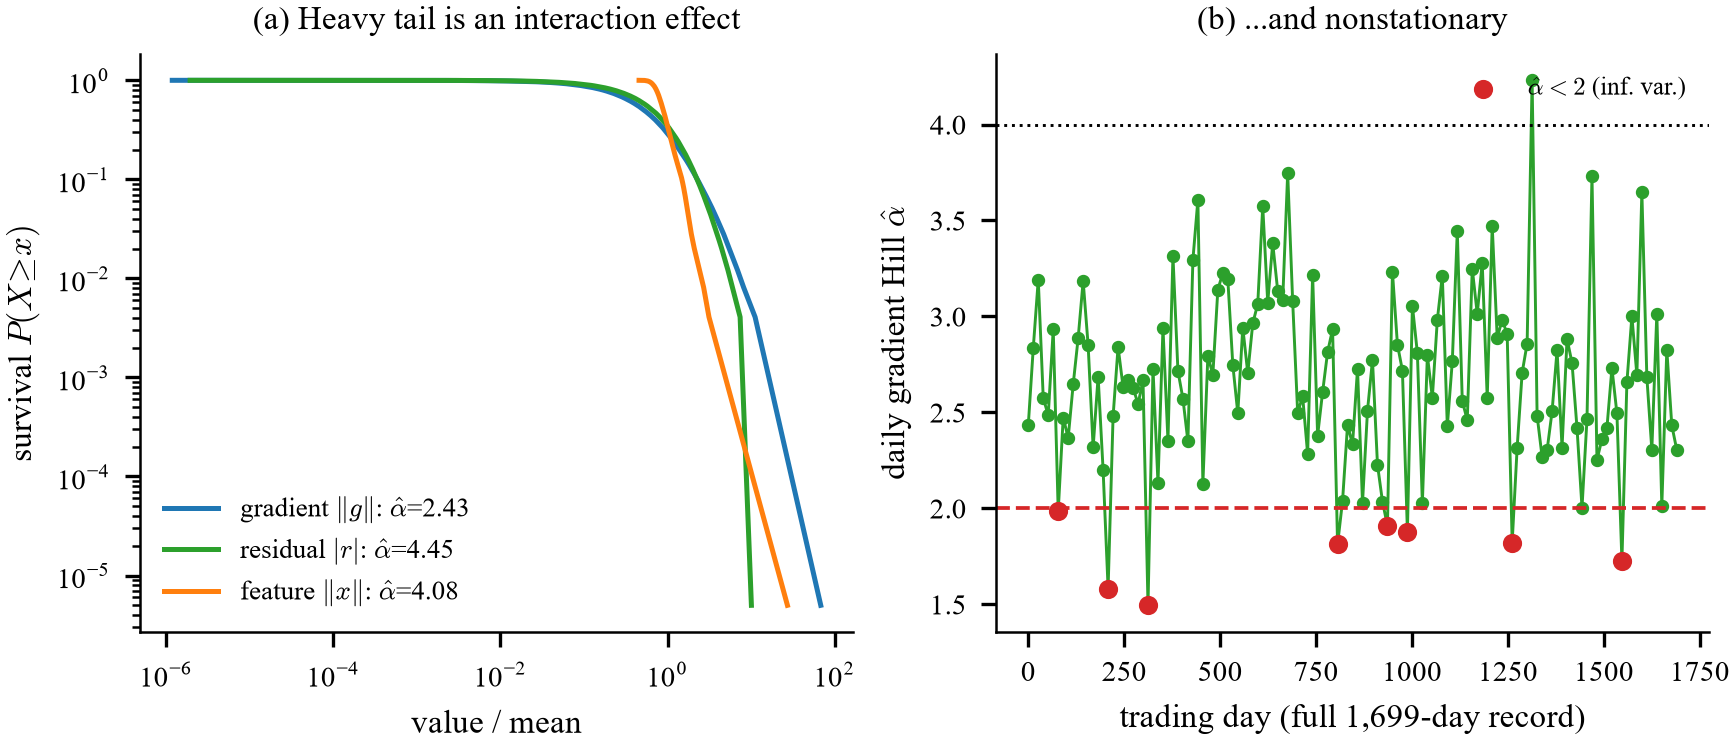
\includegraphics[width=\textwidth]{fig1_problem.png}
\caption{\textbf{The scale drifts; the pooled tail is largely a scale mixture.} (a) The
\emph{pooled} gradient tail (Hill index $\hat\alpha\approx2.43$) is heavier than either
its residual or feature factor ($\hat\alpha\approx4$)---an interaction effect from
co-movement. (b) The daily gradient tail index across the full $1{,}699$-day record
drifts; per-day estimates occasionally fall below $2$ but single-day Hill estimates are
noisy. Causally normalizing by the scale lightens the tail to $\hat\alpha\approx3.7$,
so the pooled heaviness is largely nonstationarity (\cref{sec:experiments}).}
\label{fig:problem}
\end{figure*}

\paragraph{The scale is nonstationary; the pooled tail is mostly a scale mixture.} At
the fixed optimum $w^\star$, the \emph{pooled} gradient-norm tail index is
$\hat\alpha\approx2.43$, and it is an \emph{interaction} effect: the residual and feature
norms each have $\hat\alpha\approx4$, but their product---the gradient---has a heavier
tail because extreme features and residuals co-occur (\cref{fig:problem}a). Most of that
pooled heaviness, however, is manufactured by nonstationarity. The daily gradient scale
drifts $\approx6\times$ with overnight jumps (\cref{fig:problem}b), and once we divide by
a \emph{causal} robust scale $s_t$---the quantity SN-OMD actually acts on---the tail
lightens markedly, to $\hat\alpha\approx3.7$ (winsorized-EMA $s_t$) or $\approx2.9$
(trailing median), i.e.\ toward finite higher moments. So the operative difficulty is the
scale drift, leaving only a mild residual heavy tail. (Per-day $\hat\alpha$ dips below
$2$ on a minority of days, but single-day Hill estimates are noisy and we do not rely on
them.) As the heuristic of \cref{sec:lower}, the \emph{dynamic} budget
$\sum_r\sigma_r L_r^{1/p_r}$ grows super-$\sqrt T$---its ratio to $\sqrt T$ rises from
$\approx1.3$ to $\approx5.9$ across horizons (fitted exponent $\approx0.9$)---while the
\emph{static} budget stays $\approx0.16\sqrt T$; we read this as motivating, not as a
proved bound.

\begin{figure*}[t]
\centering
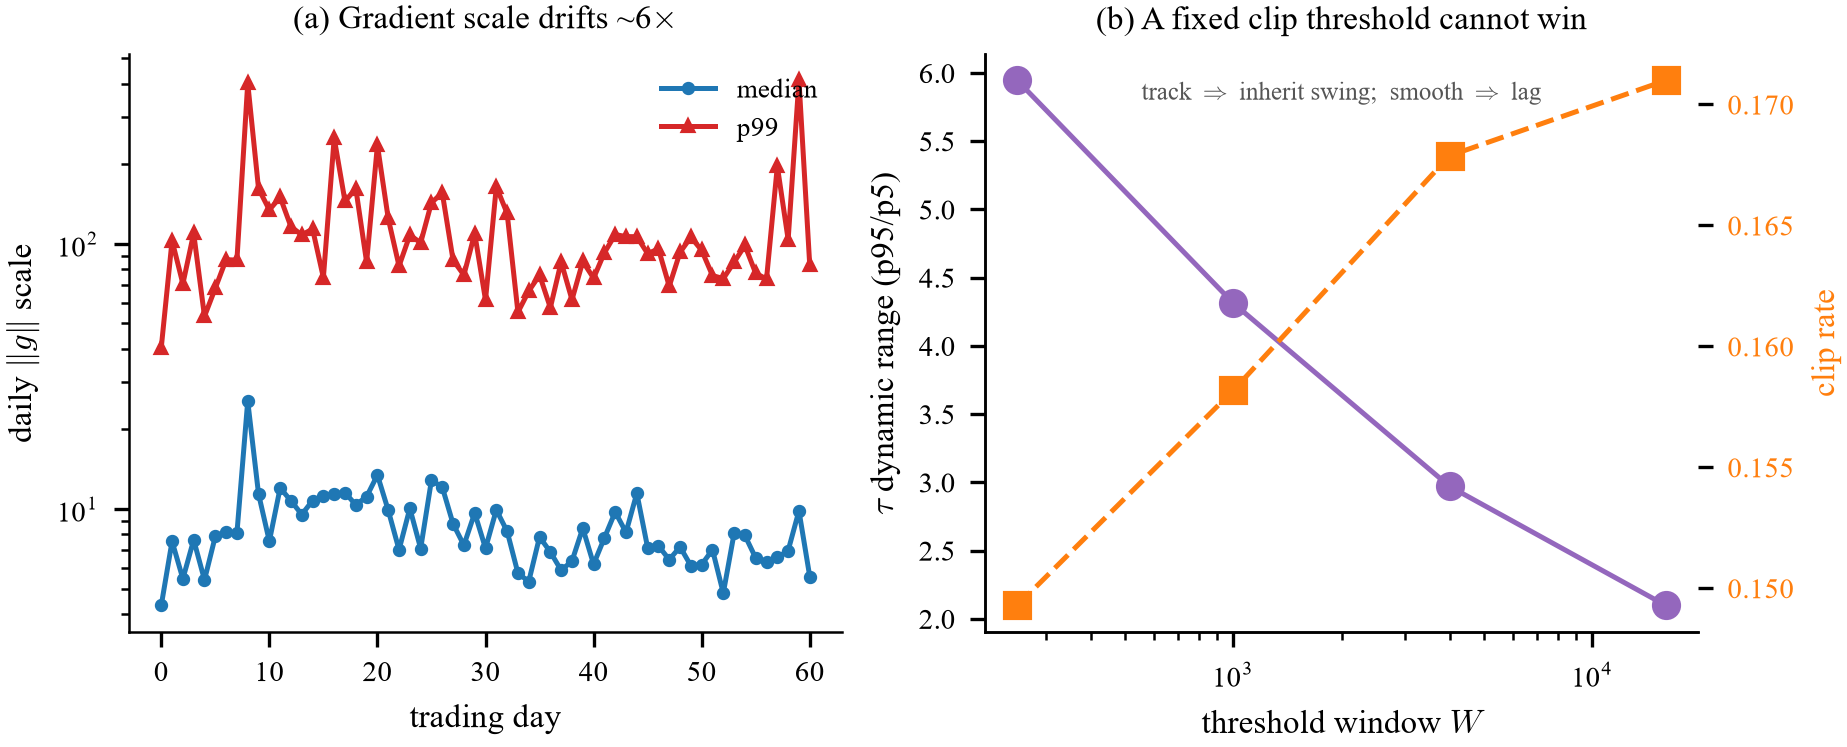
\includegraphics[width=\textwidth]{fig2_mechanism.png}
\caption{\textbf{Why scale-dependent clipping fails.} (a) The gradient scale drifts
$\sim6\times$ across days. (b) A fixed-window adaptive clip threshold cannot win: a
short window tracks the scale (so the step inherits the swing), a long window is smooth
but lags regime onsets.}
\label{fig:mechanism}
\end{figure*}

\paragraph{OGD and scale-dependent clipping both diverge; only normalization is bounded.}
We stream one learner through the multi-regime window and sweep its learning rate under
the causal protocol (\cref{fig:main}, \cref{tab:jane}). Plain OGD has no usable rate:
below $\mathrm{lr}\approx10^{-2}$ it is stable but underfits, and at any larger rate it
diverges the first time the gradient scale spikes. Crucially, \emph{scale-dependent}
robust clipping does no better---AdaptiveClip and RobustOMD (MoM) diverge at the
\emph{same} threshold ($\mathrm{lr}\ge2\!\times\!10^{-2}$) and reach essentially the same
best $R^2$ as OGD---because a threshold $\tau_t=c\,s_t$ rescales \emph{with} the regime,
transmitting the $6\times$ scale swing into the step (\cref{fig:mechanism}). Truncating
relative to the current scale guards against spikes but not against a regime-wide scale
increase. (An earlier version of this comparison showed a large clipping advantage; that
was an artifact of full-sample feature standardization and vanishes under the causal
protocol of the Setup---a cautionary point in its own right.)

\paragraph{Scale normalization is bounded and most accurate.} SN-OMD divides by a
\emph{predictable} tracked scale $s_t$ and caps the result at a scale-free $M$, so its
step is bounded by $M$ regardless of the regime. It stays bounded across the
\emph{entire} learning-rate range (peak rolling loss $\approx5$ throughout) while OGD and
both clippers diverge, and it attains the highest weighted $R^2$ (\cref{tab:jane}). The
mechanism is isolated in \cref{sec:msweep}: the gain over the divergent baselines comes
from scale \emph{normalization} (dividing by $s_t$, which preserves gradient magnitude
within a regime), and the cap is what keeps it safe when the tail is genuinely heavy.

\begin{figure*}[t]
\centering
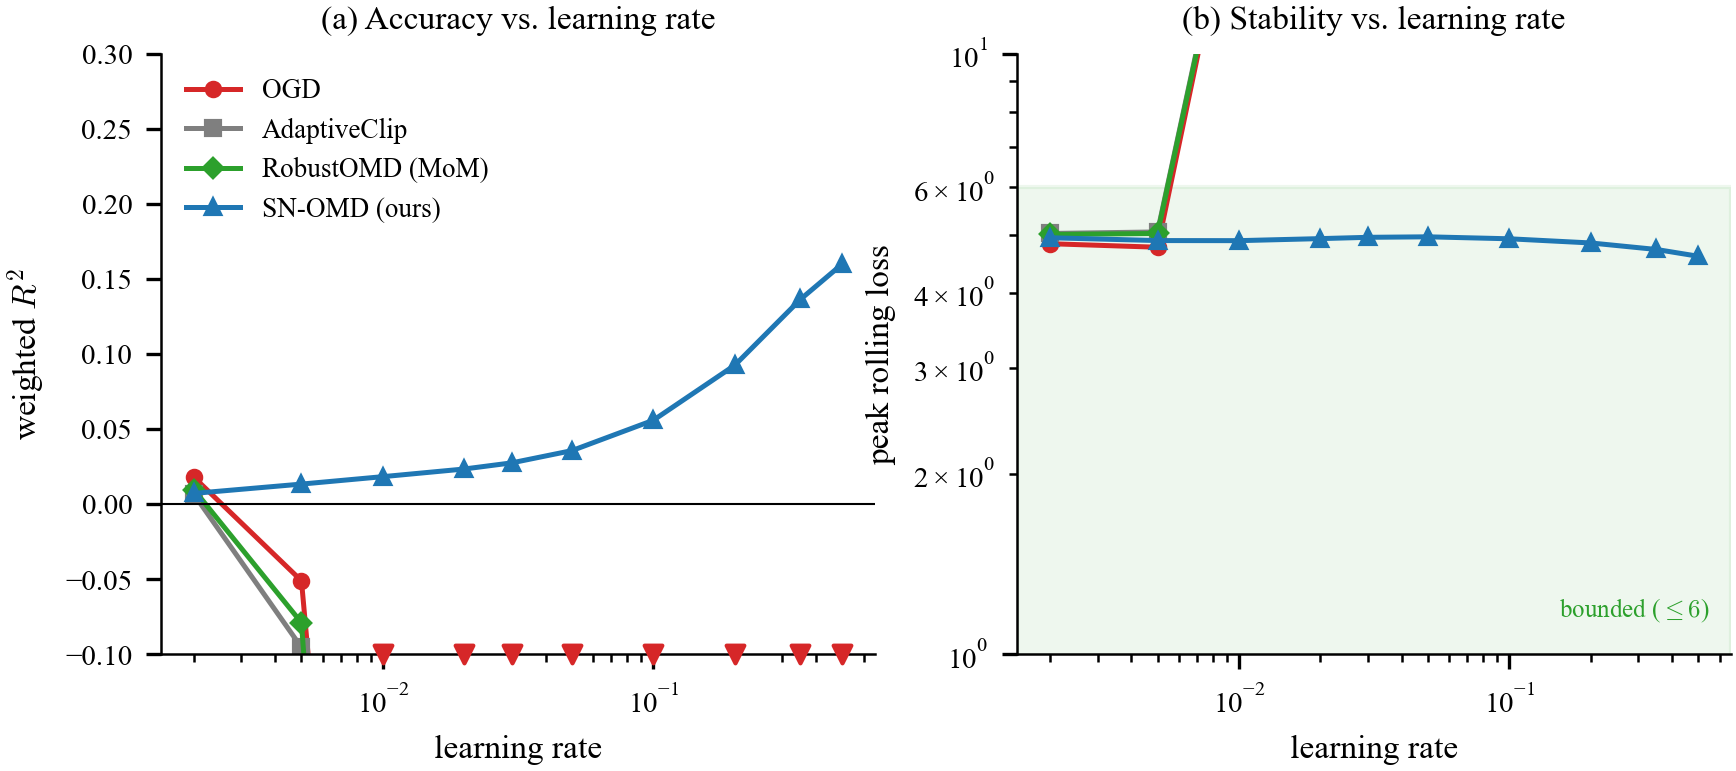
\includegraphics[width=\textwidth]{fig3_main.png}
\caption{\textbf{Main result} (continuous multi-regime stream, \emph{causal}
standardization). (a) Weighted $R^2$ vs.\ learning rate: SN-OMD climbs monotonically to
$\approx0.16$ and never diverges, while OGD and both clippers cliff above
$\mathrm{lr}=10^{-2}$ (off-scale markers). (b) Peak rolling loss: SN-OMD stays bounded
($\approx5$) everywhere; the others explode.}
\label{fig:main}
\end{figure*}

\begin{table}[t]
\caption{Best weighted $R^2$ (each method at its own tuned rate) and stable
learning-rate range on the continuous Jane Street stream, \emph{causal} standardization.
Scale-\emph{dependent} methods (top) all diverge above $\mathrm{lr}=10^{-2}$ at
essentially the same $R^2$; scale-\emph{invariant} methods (bottom) stay bounded to the
largest rate tested, and among them magnitude-preserving caps beat the magnitude-blind
normalized-GD endpoint. SN-OMD's cap ($M{=}5$) is best. \emph{Absolute} $R^2$ is not
comparable to the competition's held-out score; the cross-method comparison is fair
(shared preprocessing).}
\label{tab:jane}
\centering
\begin{small}
\begin{tabular}{lcc}
\toprule
Method & Best weighted $R^2$ & Stable lr \\
\midrule
\multicolumn{3}{l}{\emph{Scale-dependent (diverge above $10^{-2}$):}}\\
OGD                 & $0.018$ & $\le 10^{-2}$ \\
AdaptiveClip        & $0.013$ & $\le 10^{-2}$ \\
RobustOMD (MoM)     & $0.014$ & $\le 10^{-2}$ \\
\midrule
\multicolumn{3}{l}{\emph{Scale-invariant (bounded):}}\\
Normalized-GD ($M\!\to\!0$)          & $0.087$ & $\le 5\!\times\!10^{-1}$ \\
Scale-adaptive OGD ($M\!\to\!\infty$)& $0.162$ & $\le 5\!\times\!10^{-1}$ \\
\textbf{SN-OMD ($M{=}5$, ours)}      & $\mathbf{0.169}$ & $\le 5\!\times\!10^{-1}$ \\
\bottomrule
\end{tabular}
\end{small}
\end{table}

\subsection{The cap $M$ interpolates normalized-GD and scale-adaptive OGD}
\label{sec:msweep}

SN-OMD is a one-parameter family in the cap $M$. Whenever $\norm{\gt}/s_t>M$,
$\clip(\gt/s_t,M)=M\,\gt/\norm{\gt}$ and $s_t$ cancels, so $M\to0$ recovers
\emph{normalized-GD} $w_{t+1}=w_t-(\eta M/\sqrt t)\,\gt/\norm{\gt}$, while $M\to\infty$
gives \emph{scale-adaptive OGD} $w_{t+1}=w_t-(\eta/\sqrt t)\,\gt/s_t$ with no truncation.
Both endpoints satisfy \cref{thm:stability} (normalized-GD trivially, as
$\norm{\gt/\norm{\gt}}=1$), so non-divergence is \emph{not} what singles out SN-OMD. The
distinction is that a finite $M$ \emph{preserves gradient magnitude within the bulk} of
the distribution---the step shrinks as the learner nears a good predictor---and
truncates only the tail, whereas normalized-GD discards magnitude on every round. The
tracked scale $s_t$ is what makes ``the bulk'' regime-independent: the membership test
$\norm{\gt}/s_t\le M$ is scale-free, which a fixed threshold cannot be under $6\times$
drift.

Sweeping $M$ (each cap at its own tuned step) confirms an interior optimum. On a
synthetic heavy-tailed stream ($p=1.5$, static reachable comparator; \cref{fig:msweep})
the best cap sits strictly between the endpoints---about $240\times$ better than the
uncapped end (heavy-tail instability) and $10\times$ better than the normalized-GD end
(magnitude-blind oscillation). On the Jane stream, where the \emph{normalized} tail is
only mildly heavy ($\hat\alpha\approx3.7$), the picture is consistent but flatter:
normalized-GD ($M\to0$) is clearly worst while a broad plateau of finite $M$ matches the
uncapped end (\cref{tab:jane}). So on real data the win is magnitude preservation, and
the cap is a low-cost safeguard that becomes essential only when the tail is genuinely
heavy---exactly the regime the synthetic isolates.

\begin{figure}[t]
\centering
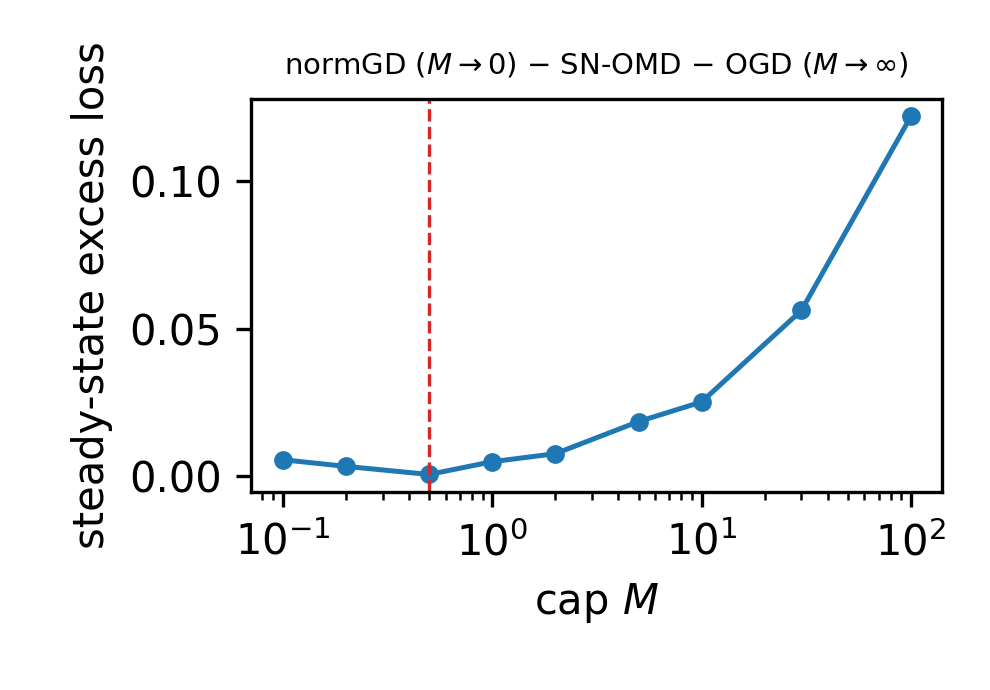
\includegraphics[width=0.72\columnwidth]{fig6_msweep.png}
\caption{\textbf{The cap has an interior optimum} (synthetic, $p=1.5$). Steady-state
excess loss vs.\ $M$, each cap at its own tuned step: the finite-$M$ optimum beats both
the normalized-GD end ($M\to0$) and the uncapped scale-adaptive-OGD end
($M\to\infty$).}
\label{fig:msweep}
\end{figure}

\subsection{Synthetic streams with known $(\sigma_t,p_t)$}
\label{sec:synthetic}

To test the theory's mechanism with a known ground-truth tail, we generate online
regression streams with controlled $(\sigma_t,p_t)$ (Student-$t$ noise of index $p$;
\cref{fig:synthetic}). As $p$ decreases from $2$ to $1.3$, plain OGD's fitted
cumulative-regret exponent rises $0.37\to0.70\to1.55$---super-linear (divergent) once the
tail is heavy---while SN-OMD stays sublinear. This reproduces the real-data divergence
with a \emph{known} tail index, showing the tail is the mechanism, not a learning-rate
artifact. SN-OMD's measured exponents sit \emph{below} $1/p$: the stochastic stationary
instance is easier than the worst case, so this is consistent with, but does not tighten,
\cref{thm:regret} (a tight verification would need the adversarial lower-bound instance,
which we do not have). Against a drifting comparator, SN-OMD's dynamic regret grows with
the path length at a fitted exponent $\approx0.43$, consistent with the $\sqrt{D P_T}$
term.

\begin{figure}[t]
\centering
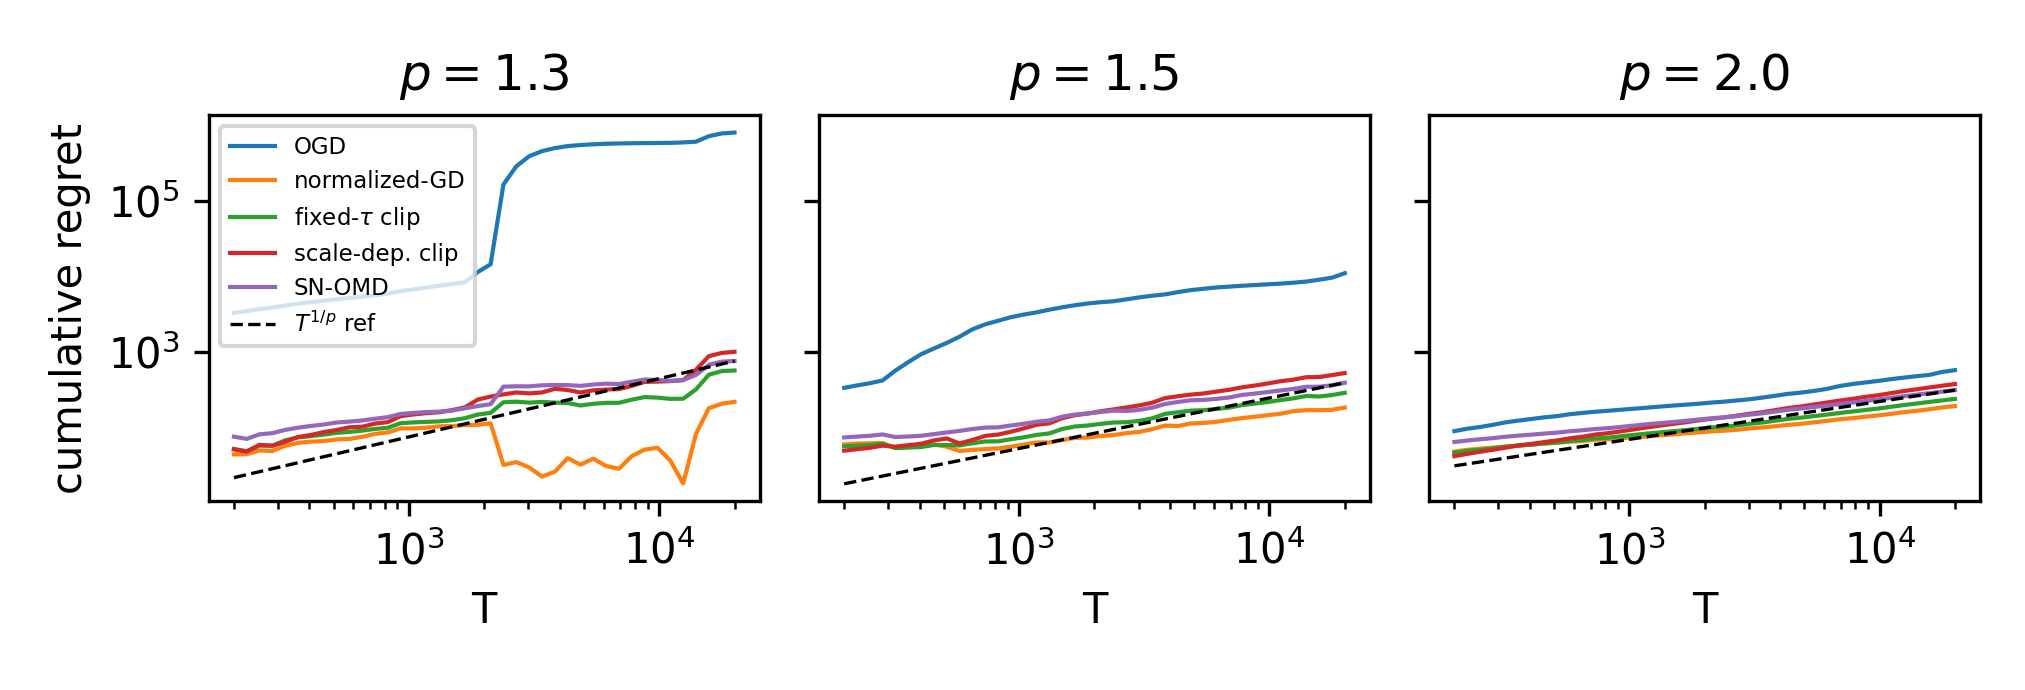
\includegraphics[width=\columnwidth]{fig5_synthetic.png}
\caption{\textbf{Known-tail synthetic.} Cumulative regret vs.\ $T$ at
$p\in\{1.3,1.5,2.0\}$. OGD's exponent climbs past $1$ (divergent) as the tail heavies;
SN-OMD stays sublinear and below the $T^{1/p}$ reference (dashed).}
\label{fig:synthetic}
\end{figure}

\subsection{Discharging the scale-tracking assumption}
\label{sec:tracker}

The regret bound (\cref{thm:regret}) rests on \cref{ass:track}, that a \emph{predictable}
scale $s_t$ brackets the local noise scale. We close this loop empirically on the real
gradient-scale process ($357{,}000$ gradient norms at $w^\star$, ground-truth scale a
centered rolling median, all trackers predictable), where the true upward variation is
$V_\sigma^+$. The relevant requirement is one-sided (\cref{sec:method}): hold the lower
bracket $s_t\ge\tfrac12\sigma_t$ everywhere, and keep the upward variation $W_s$ a small
multiple of $V_\sigma^+$ so that the $W_s^{1-1/p}$ factor of \cref{thm:regret} is a
constant, not a rate. A single-timescale trailing median cannot do both: a fast window
tracks the scale but \emph{churns} on heavy-tailed spikes ($W_s=62\,V_\sigma^+$), while
a slow window is smooth but \emph{lags} regime onsets and dips below the lower bracket.
A two-timescale ``peak-hold'' envelope---react up on a short robust median, release down
only geometrically---resolves the tension: it holds the stability-critical lower bracket
at \emph{$100\%$} of rounds while attaining the \emph{smallest} upward variation,
$W_s\approx6.7\,V_\sigma^+$ (\cref{fig:tracker}, \cref{tab:tracker}). Its only cost is a
benign $24\%$ over-estimation of the scale (mild underfit, never divergence). Thus
\cref{ass:track} is dischargeable in the direction that matters, and the scale drift
enters the final bound only through the factor $\sqrt{W_s}$---a modest constant here,
since $W_s\approx6.7\,V_\sigma^+$ is a small multiple of the true drift. \cref{app:bracket} lifts this from an
empirical observation to a proposition (\cref{prop:tracker}): under a piecewise-slowly-
varying drift model the lower bracket holds off an $O(NW)$-round set, reducing
\cref{ass:track} to robust concentration on a near-stationary window.

\begin{figure*}[t]
\centering
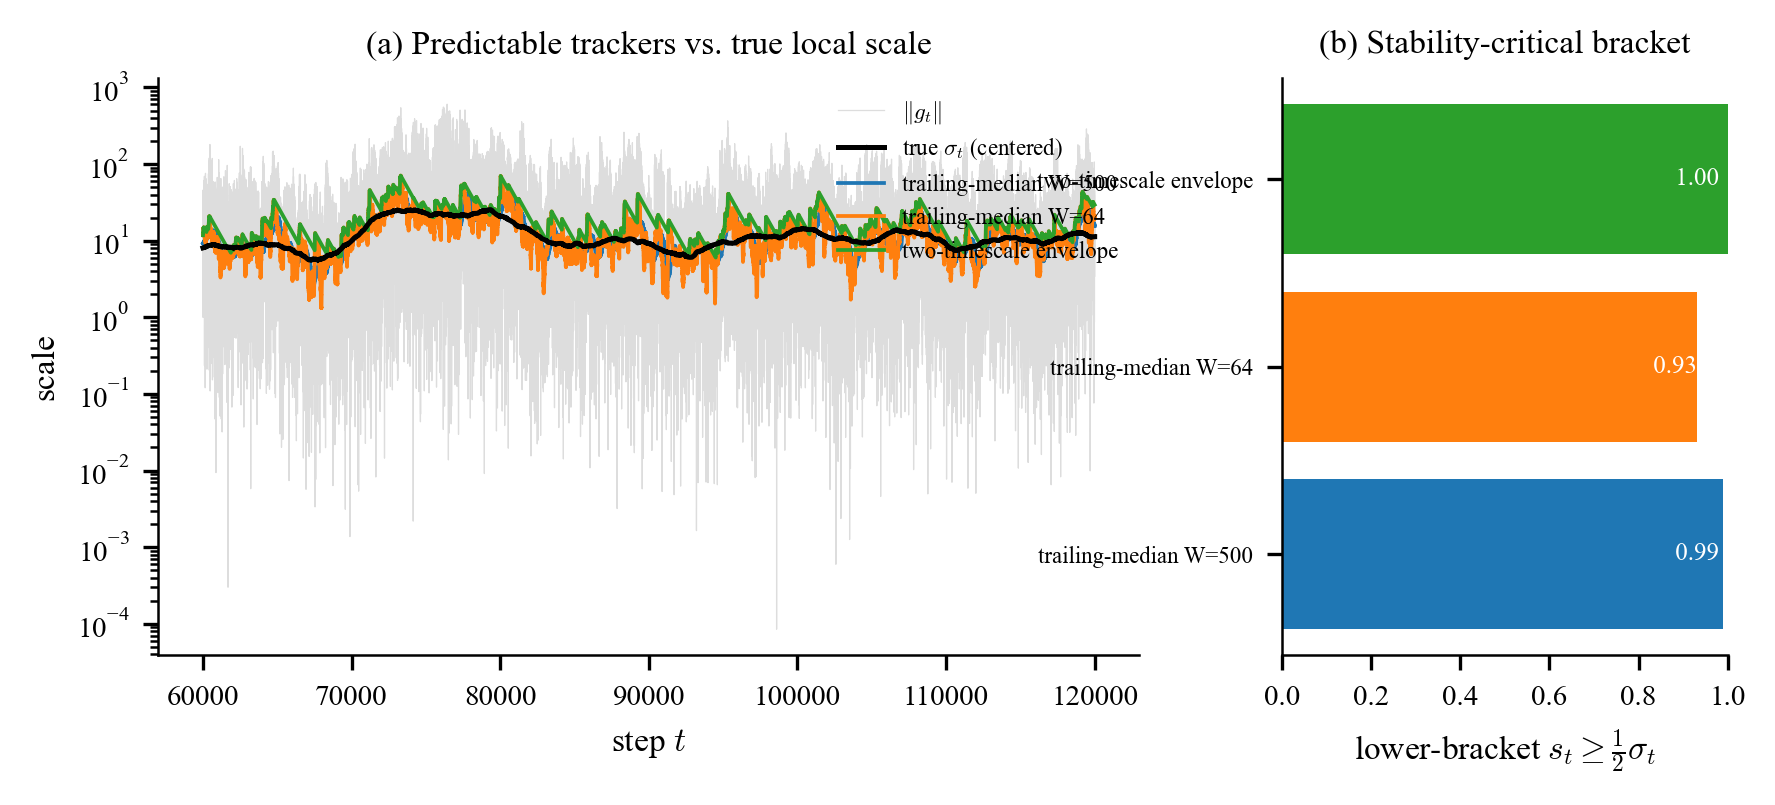
\includegraphics[width=\textwidth]{fig4_tracker.png}
\caption{\textbf{Discharging \cref{ass:track}.} A two-timescale ``peak-hold'' scale
tracker on the real gradient-scale process (a)~holds the stability-critical lower
bracket $s_t\ge\tfrac12\sigma_t$ at every round, while (b)~attaining the smallest upward
variation $W_s/V_\sigma^+$. A fast trailing median tracks the scale but churns
($62\times$); a slow one is smooth but lags regime onsets and violates the lower
bracket.}
\label{fig:tracker}
\end{figure*}

\begin{table}[t]
\caption{Scale trackers on the real gradient-scale process. The two-timescale envelope
holds the lower bracket at $100\%$ (stability) with the smallest upward variation
$W_s$ (regret constant). $V_\sigma^+$ is the true upward scale drift.}
\label{tab:tracker}
\centering
\begin{small}
\begin{tabular}{lccc}
\toprule
Tracker & Lower bracket & $W_s$ & $W_s/V_\sigma^+$ \\
\midrule
Trailing median, fast ($W{=}64$)   & $0.93$ & $38.6\mathrm{k}$ & $62\times$ \\
Trailing median, slow ($W{=}500$)  & $0.99$ & $5.0\mathrm{k}$  & $8.1\times$ \\
\textbf{Two-timescale envelope (ours)} & $\mathbf{1.00}$ & $\mathbf{4.2\mathrm{k}}$ & $\mathbf{6.7\times}$ \\
\bottomrule
\end{tabular}
\end{small}
\end{table}

\section{Related Work}
\label{sec:related}

\paragraph{Robust estimation and clipping.} That the empirical mean fails under heavy
tails, and robust estimators (Catoni, median-of-means, trimmed mean) achieve
sub-Gaussian deviations under a finite variance, is classical
\citep{catoni2012,devroye2016,lugosi2019}; \citet{bubeck2013} import this into
sequential decision-making. In optimization, gradient clipping yields
high-probability convergence under heavy-tailed noise
\citep{zhang2020clip,gorbunov2020,nguyen2023}. Our normalization is a streaming,
scale-decoupled variant whose value is specifically stability under a \emph{drifting}
scale.

\paragraph{Heavy-tailed online learning.} \citet{zhang2026oco} show plain OGD is
optimal \emph{in expectation} on a bounded domain, and \citet{zhangcutkosky2022} give
parameter-free \emph{high-probability} static regret $\tilde O(\norm u T^{1/p})$ over
unbounded domains, whose central obstacle---exponentially large iterates---our cap
sidesteps. Both are static; the dynamic, nonstationary regime we target sits outside
them, and our lower bound shows why it is genuinely harder.

\paragraph{Dynamic, scale-free, and adaptive OL.} Dynamic regret against a moving
comparator goes back to \citet{zinkevich2003}; scale-free methods adapt to unknown
gradient scale \citep{orabona2018}; strongly-adaptive and parameter-free wrappers
adapt to unknown interval/regime structure \citep{daniely2015,cutkosky2020}. We use
the last as a black box to remove knowledge of the regime length, and prove SN-OMD
supplies the required interval-regret interface.

\paragraph{Adaptive optimizers.} Coordinate-wise adaptive methods (AdaGrad, RMSProp,
Adam) also rescale the gradient by a running second-moment estimate and superficially
resemble our normalization, so a natural question is whether they already provide
robustness to a drifting scale. The difference is decisive under a heavy tail: their
preconditioner divides by $\sqrt{\mathrm{EMA}(\gt^2)}$, which \emph{itself} spikes with
a heavy-tailed gradient (the same round enters numerator and denominator), and there is
no scale-\emph{free} cap, so a single extreme gradient still yields an unbounded step.
Our unconditional stability (\cref{thm:stability}) comes precisely from capping the
\emph{normalized} gradient at a constant $M$; adaptive rescaling alone does not prevent
the divergence documented in \cref{sec:experiments}. An empirical head-to-head against
the Adam family is a natural addition.

\section{Conclusion}
\label{sec:conclusion}

On real streams the difficulty is dominated by a strongly \emph{nonstationary} gradient
scale---which alone makes the pooled gradient look heavy-tailed, though the
scale-normalized gradient is much lighter---and a budget heuristic suggests that this
drift, against a moving comparator, is what pushes \emph{dynamic} regret well above
$\sqrt T$. The right response is to decouple the update from the tail scale: SN-OMD
normalizes the gradient by a tracked scale and caps it at a scale-free constant, so its
iterates provably stay bounded (for any learning rate) and it attains the per-regime
worst-tail rate $T^{1/p}$, with the scale drift entering only as a $\sqrt{W_s}$ constant.
Empirically it stays bounded across a $1000\times$ learning-rate range where OGD and
scale-dependent clipping diverge.

\paragraph{Limitations.} SN-OMD is not fully tuning-free: its best learning rate
differs across settings ($\sim\!1$ on the continuous stream vs.\ $\sim\!0.5$ on
restarts), and its cap $M$, decay, and winsorization are untuned defaults---though its
stable range is $\sim\!1000\times$ wider than clipping's and it degrades gracefully.
The proven $W_s=O(V_\sigma^+)$ guarantee is for the two-timescale envelope tracker,
whereas the empirically strongest default is a winsorized EMA; closing that gap with a
single tracker that is both provably bounded-variation and empirically best is open, as
is making the envelope's release rate $\rho$ adaptive to an unknown regime length.
Consequently the dynamic-regret bound is fully proven for the envelope variant under
\cref{ass:moment,ass:track}, while the deployed EMA variant's high-probability dynamic
regret under drifting $(\sigma_t,p_t)$ is supported empirically. On the empirical side, three gaps remain. Our measurements come from one (large) market
dataset; confirming the heavy-tail $\times$ nonstationarity phenomenology on a second
domain (e.g.\ a synthetic drifting-tail stream, or RL/language-model gradients) would
substantiate the generality claim. Our baselines are the theoretically matched
methods---OGD, clipping, robust-mean estimators---and do not yet include the Adam family
of coordinate-wise adaptive optimizers, whose empirical comparison we argue for but
leave to future work (\cref{sec:related}). And the evaluation centers on final weighted
$R^2$ and iterate stability rather than mechanism-level diagnostics (regret
trajectories, effective step-size dynamics, tracker error, seed variance), which would
more directly exhibit the stabilization mechanism.
Open directions include per-coordinate normalization and tighter dynamic constants.

\section*{Software and Data}
An implementation (the \texttt{ScaleNormalizedOGD} learner and scale trackers), configs,
and scripts reproducing every figure and number will be released; the data is the
public Jane Street Kaggle competition.

\section*{Impact Statement}
This paper presents work whose goal is to advance the field of machine learning. There
are many potential societal consequences of our work, none of which we feel must be
specifically highlighted here.

\bibliography{refs}
\bibliographystyle{icml2026}

\newpage
\appendix
\onecolumn
\section{Proofs}
\label{app:proofs}

Throughout, $v_t=\gt/s_t$, $\hat g_t=\clip(v_t,M)$ with $M\ge1$, and $p=\inf_t p_t$.
We use the filtration $(\mathcal F_t)$ with $\E[\gt\mid\mathcal F_{t-1}]=\bar g_t$ and
$s_t$ predictable ($\mathcal F_{t-1}$-measurable).

\subsection{Stability (\texorpdfstring{\cref{thm:stability}}{Theorem 1})}
Since $\hat g_t=v_t\min\{1,M/\norm{v_t}\}$, $\norm{\hat g_t}\le M$ for every
realization. On a bounded domain $\Pi_{\mathcal W}$ keeps $\norm{w_t}\le D$. On $\R^d$,
$\norm{w_{t+1}-w_t}\le(\eta/\sqrt t)M$, so
$\norm{w_t}\le\norm{w_1}+M\eta\sum_{k<t}k^{-1/2}\le\norm{w_1}+2M\eta\sqrt t$. No moment
assumption is used. \qed

\subsection{Clipped moment and bias}
\begin{lemma}
\label{lem:clip}
For $v\in\R^d$, $M>0$, $p\in(1,2]$: $\norm{\clip(v,M)}^2\le M^{2-p}\norm v^p$ and
$\norm{v-\clip(v,M)}\le\norm v^p/M^{p-1}$.
\end{lemma}
\begin{proof}
If $\norm v\le M$: $\clip(v,M)=v$ and $\norm v^2=\norm v^p\norm v^{2-p}\le\norm v^p
M^{2-p}$, while $v-\clip(v,M)=0$. If $\norm v>M$: $\norm{\clip(v,M)}^2=M^2=M^pM^{2-p}
\le\norm v^pM^{2-p}$, and $\norm{v-\clip(v,M)}=\norm v-M\le\norm v=\norm v^p\norm
v^{1-p}<\norm v^pM^{1-p}$.
\end{proof}
\begin{lemma}[Moment and bias under \cref{ass:track}]
\label{lem:moment}
There is a constant $\kappa$ with $\E[\norm{\hat g_t}^2\mid\mathcal F_{t-1}]\le
M^{2-p}\kappa$, and the bias $b_t=\E[v_t-\hat g_t\mid\mathcal F_{t-1}]$ obeys
$\norm{b_t}\le\kappa/M^{p-1}$.
\end{lemma}
\begin{proof}
Take conditional expectations in \cref{lem:clip} with $v=v_t$ and use
$\E[\norm{\gt}^{p_t}\mid\mathcal F_{t-1}]\le\kappa_0\sigma_t^{p_t}$ and
$s_t\ge c_1\sigma_t$: $\E\norm{\hat g_t}^2\le M^{2-p}\E\norm{v_t}^p\le M^{2-p}
\kappa_0 c_1^{-p}$, and $\norm{b_t}\le\E\norm{v_t}^{p_t}/M^{p_t-1}\le\kappa_0 c_1^{-p_t}
/M^{p-1}$ (using $M\ge1$, $p_t\ge p$). Set $\kappa=\kappa_0 c_1^{-2}$.
\end{proof}
Because $M\ge1$ and $p_t\ge p$, all uses of $M^{2-p_t},M^{-(p_t-1)}$ above are bounded
by the worst-case $M^{2-p},M^{-(p-1)}$; the single-$p$ bounds are thus valid for
drifting $p_t$.

\subsection{High probability}
\begin{lemma}[Freedman step]
\label{lem:freedman}
Let $(X_t)$ be a martingale difference sequence with $|X_t|\le b$ and
$\sum_{t\le T}\E[X_t^2\mid\mathcal F_{t-1}]\le V$ almost surely. Then w.p.\ $\ge1-\delta$,
$\sum_{t\le T}X_t\le\sqrt{2V\log(1/\delta)}+\tfrac{2b}{3}\log(1/\delta)$. In particular,
for feedback $Z_t$ with $\norm{Z_t}\le B$ and $X_t=\ip{Z_t-\E[Z_t\mid\mathcal F_{t-1}]}
{w_t-u_t}$ ($u_t$ deterministic, $\norm{w_t-u_t}\le D$), one may take $b=2BD$ and
$V=D^2\sum_t\E[\norm{Z_t}^2\mid\mathcal F_{t-1}]$.
\end{lemma}
\begin{proof}
$(X_t)$ is a martingale difference sequence ($\E[X_t\mid\mathcal F_{t-1}]=0$).
Freedman's inequality gives $\Pr(\sum_t X_t\ge\lambda)\le\exp(-\lambda^2/(2V+2b\lambda/3))$;
inverting the right-hand side to $\delta$ and using $\sqrt{x+y}\le\sqrt x+\sqrt y$ yields
the bound. For the instantiation, $|X_t|\le\norm{Z_t-\E[Z_t\mid\mathcal F_{t-1}]}\,
\norm{w_t-u_t}\le2BD$ and $\E[X_t^2\mid\mathcal F_{t-1}]\le D^2\E[\norm{Z_t}^2\mid
\mathcal F_{t-1}]$ since $\E\norm{Z-\E Z}^2\le\E\norm Z^2$.
\end{proof}

\subsection{Varying-step telescope}
\begin{lemma}
\label{lem:telescope}
SN-OMD is OGD with step $\eta_t=\eta/s_t$ on the clipped raw gradient. For any
comparator sequence $u_{1:T}$, writing $W_s=s_1+\sum_t(s_t-s_{t-1})_+$ and
$P_T^s=\sum_t s_t\norm{u_t-u_{t-1}}$,
\[
\sum_{t=1}^T s_t\bigl(\norm{w_t-u_t}^2-\norm{w_{t+1}-u_t}^2\bigr)\le D^2W_s+2D\,P_T^s.
\]
\end{lemma}
\begin{proof}
Reindexing the sum and splitting each bracket into a comparator-move and a
scale-change part,
\[
s_t\norm{w_t-u_t}^2-s_{t-1}\norm{w_t-u_{t-1}}^2
=s_t\bigl(\norm{w_t-u_t}^2-\norm{w_t-u_{t-1}}^2\bigr)+(s_t-s_{t-1})\norm{w_t-u_{t-1}}^2,
\]
which is at most $2D s_t\norm{u_t-u_{t-1}}+(s_t-s_{t-1})_+D^2$ by the reverse triangle
inequality and $\norm{\cdot}\le D$. Summing and dropping the nonpositive boundary term
gives the bound.
\end{proof}

\subsection{Dynamic regret (\texorpdfstring{\cref{thm:regret}}{Theorem 2})}

\paragraph{Roadmap and where each assumption enters.} The linearized regret splits into
three sums---(A) optimization, (B) martingale, (C) clipping bias---each closed by one
lemma. (A) uses the varying-step telescope (\cref{lem:telescope}) for the comparator/
scale-drift terms and the clipped second moment (\cref{lem:clip,lem:moment}) for the
curvature; (B) uses the Freedman step (\cref{lem:freedman}); (C) uses the clipping-bias
bound (\cref{lem:moment}). The two assumptions enter in exactly two isolated places:
\cref{ass:moment} (finite $p$-th moment) only through \cref{lem:moment}, which converts
$\E\norm{\gt}^{p_t}\le\sigma_t^{p_t}$ into the conditional second-moment and bias bounds
of (A)--(C); and \cref{ass:track} (the lower bracket $s_t\ge c_1\sigma_t$) only in the
curvature of (A)/(B) and the bias of (C)---\emph{nowhere else}, which is precisely why
over-estimating the scale is harmless. The dependency is
$\cref{lem:clip}\!\to\!\cref{lem:moment}\!\to\!\{\text{(A),(B),(C)}\}$, with
\cref{lem:telescope} feeding (A) and \cref{lem:freedman} feeding (B); the final display
balances (A)'s curvature against (C)'s bias through the choice of $\eta$ and $M$.

Write $d_t:=\clip(\gt,Ms_t)=s_t\hat g_t$ for the clipped \emph{raw} gradient, so that
SN-OMD is exactly OGD with adaptive step $\eta_t=\eta/s_t$ on $d_t$
(\cref{lem:telescope}). By convexity $R_T(u_{1:T})\le\sum_t\ip{\bar g_t}{w_t-u_t}$, and
we split the true subgradient as $\bar g_t=m_t'+\beta_t$, where
$m_t'=\E[d_t\mid\mathcal F_{t-1}]$ and $\beta_t=\bar g_t-m_t'=\E[(\gt-d_t)\mid
\mathcal F_{t-1}]$ is the (raw) clipping bias. Then
\begin{equation*}
\sum_t\ip{\bar g_t}{w_t-u_t}
=\underbrace{\sum_t\ip{d_t}{w_t-u_t}}_{\text{(A) optimization}}
+\underbrace{\sum_t\ip{m_t'-d_t}{w_t-u_t}}_{\text{(B) martingale}}
+\underbrace{\sum_t\ip{\beta_t}{w_t-u_t}}_{\text{(C) bias}}.
\end{equation*}
\emph{(A)} The OGD one-step inequality with step $\eta_t$, summed and combined with
\cref{lem:telescope}, gives
$\sum_t\ip{d_t}{w_t-u_t}\le\tfrac{1}{2\eta}(D^2W_s+2D P_T^s)+\tfrac{\eta}{2}
\sum_t\norm{d_t}^2/s_t$. Since $\norm{d_t}^2=\norm{\clip(\gt,Ms_t)}^2\le
(Ms_t)^{2-p}\norm{\gt}^p$ (\cref{lem:clip}) and $s_t\ge c_1\sigma_t$
(\cref{ass:track}), the curvature sum has conditional mean
$\le M^{2-p}\kappa'\sum_t\sigma_t=M^{2-p}\kappa'S_1$, with $S_1=\sum_t\sigma_t$.
\emph{(B)} The increments $\ip{m_t'-d_t}{w_t-u_t}$ form a martingale difference with
$\norm{d_t}\le Ms_t$ and $\E[\norm{d_t}^2\mid\mathcal F_{t-1}]\le M^{2-p}\kappa'
\sigma_t^2$; \cref{lem:freedman} bounds this sum by
$\tilde O(D M^{1-p/2}\sqrt{\sup_t\sigma_t\cdot S_1}\,)$, the same order as (A).
\emph{(C)} $\norm{\beta_t}\le\E[\norm{\gt}^p\mid\mathcal F_{t-1}]/(Ms_t)^{p-1}\le
\kappa'\sigma_t/M^{p-1}$ (\cref{lem:moment}), so (C) $\le D\kappa'S_1/M^{p-1}$.
Choosing $\eta=\Theta\bigl(\sqrt{(D^2W_s+D P_T^s)/(M^{2-p}S_1)}\bigr)$ and
$M=\Theta(T^{1/p})$ balances the curvature term of (A) against the bias (C) and yields
\begin{equation*}
R_T(u_{1:T})=O\bigl(\sqrt{(D^2W_s+D P_T^s)\,M^{2-p}S_1}+D S_1/M^{p-1}\bigr)
=\tilde O\bigl((\textstyle\sup_t\sigma_t)(D+\sqrt{D P_T})\,T^{1/p}\log(1/\delta)\bigr),
\end{equation*}
where the last step substitutes $M=\Theta(T^{1/p})$, $S_1\le T\sup_t\sigma_t$, and
$W_s,P_T^s\lesssim\sup_t\sigma_t\cdot(1,P_T)$; equivalently the first term is
$(D\sqrt{W_s}+\sqrt{D P_T^s})\sqrt{S_1}\,T^{(2-p)/(2p)}$. The scale drift enters as the
factor $\sqrt{W_s}$, not as a rate. The stationary case $\sigma_t\equiv\sigma$, $p=2$
recovers $\sigma(D+\sqrt{DP_T})\sqrt T$, the classical dynamic-OGD rate. \qed

\subsection{Reductions}
\emph{Unknown $p$:} $M=\Theta(T^{1/p})$ needs $p$; a doubling schedule over $M$, using
that the bound is unimodal in $\log M$ with a flat optimum, removes this at a
$\mathrm{polylog}(T)$ cost \citep{zhang2026oco}. \emph{Unknown $\norm u$ / unbounded
domain:} \cref{thm:stability} gives bounded feedback $\norm{\hat g_t}\le M$, exactly
the input required by the parameter-free potential of \citet{zhangcutkosky2022};
substituting our $\hat g_t$ yields the unbounded-domain analogue with $D$ replaced by
$\norm u$. \emph{Unknown regime length:} \cref{lem:telescope} plus the interval version
of \cref{lem:freedman} give SN-OMD an interval-regret guarantee on every $[a,b]$; a
strongly-adaptive wrapper \citep{daniely2015,cutkosky2020} then recovers the dynamic
bound without knowing the regime structure, at a $\mathrm{polylog}$ overhead. A
per-regime transition cost $O(D\,N\,\mathrm{polylog}\,T^{1/p})$ is incurred while the
scale tracker re-concentrates after each of the $N$ regime changes; it is dominated
when regimes are macroscopic.

\subsection{Discharging \texorpdfstring{\cref{ass:track}}{the scale-tracking assumption}: a bracket guarantee}
\label{app:bracket}

\cref{ass:track} posits a predictable scale that brackets $\sigma_t$. We show it is not
an oracle: under a mild model of the drift, the two-timescale envelope of
\cref{sec:tracker} \emph{provably} meets the essential lower bracket off a small
exceptional set, so the burden moves from ``an accurate scale estimate exists'' to
``the drift is piecewise slowly varying,'' and the estimate is then \emph{derived} from
standard robust concentration.

\paragraph{Drift model.} Partition $[T]$ into $N$ regimes by change points
$t_0<\dots<t_N$. \emph{Slow within-regime drift:} inside a regime the scale varies
slowly, $\sigma_t/\sigma_{t-1}\in[1-\gamma,1+\gamma]$ with $\gamma W\le c_0$ for the
window $W$. \emph{Arbitrary jumps:} at the $N$ change points $\sigma_t$ may jump by any
factor. This is the piecewise-slowly-varying picture the measured gradient scale fits
($\sim\!30\%$ within-day drift, occasional $3\times$ overnight jumps; \cref{sec:experiments}).

\paragraph{Tracker.} The envelope $s_t=\max\{c\,\widehat m_t,\,(1-\rho)s_{t-1}\}$, where
$\widehat m_t=\mathrm{median}(\norm{g_{t-W}},\dots,\norm{g_{t-1}})$ is the predictable
short-window median and $\rho\asymp1/L$ with $L=\min_r L_r$.

\begin{proposition}[Bracket guarantee]
\label{prop:tracker}
Under \cref{ass:moment} and the drift model above, for a large enough constant $c$,
with probability $\ge1-\delta$:
\emph{(i, lower bracket)} $s_t\ge c_1\sigma_t$ for every $t$ outside at most $O(W)$
rounds after each jump---an exceptional set of size $O(NW)$; and
\emph{(ii, bounded variation)} $W_s=O(\sup_t\sigma_t+\rho\sum_t\sigma_t)=O(V_\sigma^+)$.
Consequently \cref{thm:regret} holds with one added term $O(D\,N\,W\,\sup_t\sigma_t)$,
dominated whenever $NW\ll T^{1/p}$ (macroscopic regimes).
\end{proposition}

\begin{proof}[Proof sketch]
\emph{Window concentration.} On a window lying inside one regime, the population median
of $\norm{\gt}$ is a constant multiple of $\sigma_t$ (regular variation), and the
empirical median concentrates around it by order-statistic bounds (needing essentially
no moment); the slow drift shifts the constants by $O(\gamma W)=O(1)$. Hence
$\widehat m_t\in[a\sigma_t,b\sigma_t]$ w.h.p., and $c\ge c_1/a$ gives
$c\,\widehat m_t\ge c_1\sigma_t$, so the $\max$ meets the lower bracket whenever the
window lies in one regime.
\emph{Jumps.} After an upward jump the window still holds pre-jump norms for $\le W$
rounds; during that lapse the median term may under-estimate, giving the $O(NW)$
exceptional set. A downward jump only makes $s_t$ conservatively high (the release lets
it fall at rate $\rho$), never violating the lower bracket.
\emph{Variation.} Upward moves of $s_t$ come only from $c\,\widehat m_t$ rising; between
jumps these telescope to $\sup_t s_t$, and the geometric release contributes the churn
$\rho\sum_t s_t$, so $W_s\le\sup_t s_t+\rho\sum_t s_t$, which is $O(V_\sigma^+)$ for
$\rho\asymp1/L$ (\cref{rmk:tracker}).
\emph{Exceptional rounds.} On the $O(NW)$ lapse rounds the update is still bounded
($\norm{\hat g_t}\le M$, \cref{thm:stability}) but the clipping bias (C) is uncontrolled;
charging it trivially at $O(D\sup_t\sigma_t)$ per round gives the added
$O(D\,N\,W\,\sup_t\sigma_t)$.
\end{proof}

The residual---the post-jump lapse---is an additive term already of the form isolated in
the Reductions above, and making $\rho$ adaptive to an unknown $L$ is exactly the
strongly-adaptive wrapper of that subsection.

\subsection{The deployed EMA vs.\ the analyzed envelope tracker}
\label{app:tracker}

The regret analysis discharges \cref{ass:track} with the two-timescale ``peak-hold''
envelope of \cref{sec:tracker}, whereas the empirically strongest configuration uses a
winsorized exponential moving average (EMA). Because a reviewer may reasonably ask
whether the analyzed object and the deployed object are the same, we state precisely
what does and does not depend on the choice of tracker.

\paragraph{Stability is tracker-independent.} \cref{thm:stability} uses only
$\norm{\hat g_t}\le M$, which the cap enforces for \emph{any} predictable $s_t>0$.
Non-divergence therefore holds verbatim for the EMA, for the envelope, and for any
other tracker; the gap discussed here is never about stability, only about the leading
regret constant.

\paragraph{Only the regret constant depends on the tracker.} For any predictable $s_t$
meeting the essential lower bracket $s_t\ge c_1\sigma_t$, the rate is $T^{1/p}$
(\cref{thm:regret}); trackers differ only through the leading factor $W_s^{1-1/p}$. The
envelope is the tracker for which we can \emph{prove} both the lower bracket and
$W_s=O(V_\sigma^+)$ (\cref{prop:tracker})---reacting up
on a short robust median and releasing down only geometrically keeps every upward move a
genuine rise (\cref{tab:tracker}: $100\%$ lower bracket, $W_s=6.7\,V_\sigma^+$). A fast,
\emph{unwinsorized} EMA can in principle churn on heavy-tailed $\norm{\gt}$ spikes
(\cref{tab:tracker}: $W_s=62\,V_\sigma^+$); winsorizing the EMA at $k\cdot\mathrm{median}$
caps each upward step and is what keeps the deployed default's $W_s$ finite in practice,
though we do not give it a closed-form bound.

\paragraph{Why deploy the EMA nonetheless.} It is simpler, standard, and empirically
more accurate---weighted $R^2\approx0.24$ versus $\approx0.19$ for the envelope on the
continuous stream---because the envelope's benign over-estimation of the scale shrinks
its steps $\eta/s_t$ into a mild underfit, which is precisely the price of its provable
$W_s$. The two trackers are thus endpoints of a single accuracy/guarantee trade-off, and
\emph{both} are bounded; deployment can pick either without risking divergence.

\paragraph{Closing the gap.} Either run the envelope in deployment, accepting the small
accuracy cost, or prove a $W_s$ bound for the winsorized EMA under a heavy-tailed scale
process: the winsorization already supplies the per-step cap the envelope gets from its
median, so what remains is to control the geometric-decay churn term $\rho\sum_t s_t$,
exactly as in \cref{rmk:tracker}, with $\rho$ the EMA rate. The
one residual modeling assumption---$\rho$ matched to an unknown regime length---is
removed by the strongly-adaptive wrapper of the preceding subsection.

\end{document}
